\section{Umsetzung der einzelnen Module}
Der Kern unserer Idee ist die Richtungsbestimmung, die aus den Phasendifferenzen der verschiedenen Wellen bei verschiedenen Mikrofonen eine Richtung berechnet. Um diese Komponente überprüfen und das Verfahren anwenden zu können, haben wir die verschiedenen Module implementiert (Siehe Abbildung \ref{fig:flowchart}). Hierbei haben wir diese wie vorgesehen so universell umgesetzt, dass wir das Richtungsbestimmungsmodul sowohl mithilfe einer Simulation als auch mithilfe eines praktischen Aufbaus evaluieren können. Das nachfolgende Kapitel beschreibt eben diese Umsetzung in der Reihenfolge, mit der das Signal verarbeitet wird; von der Aufnahme der Schallquellen bis zur Ausgabe der Positionsdaten.
\begin{figure}[H]
	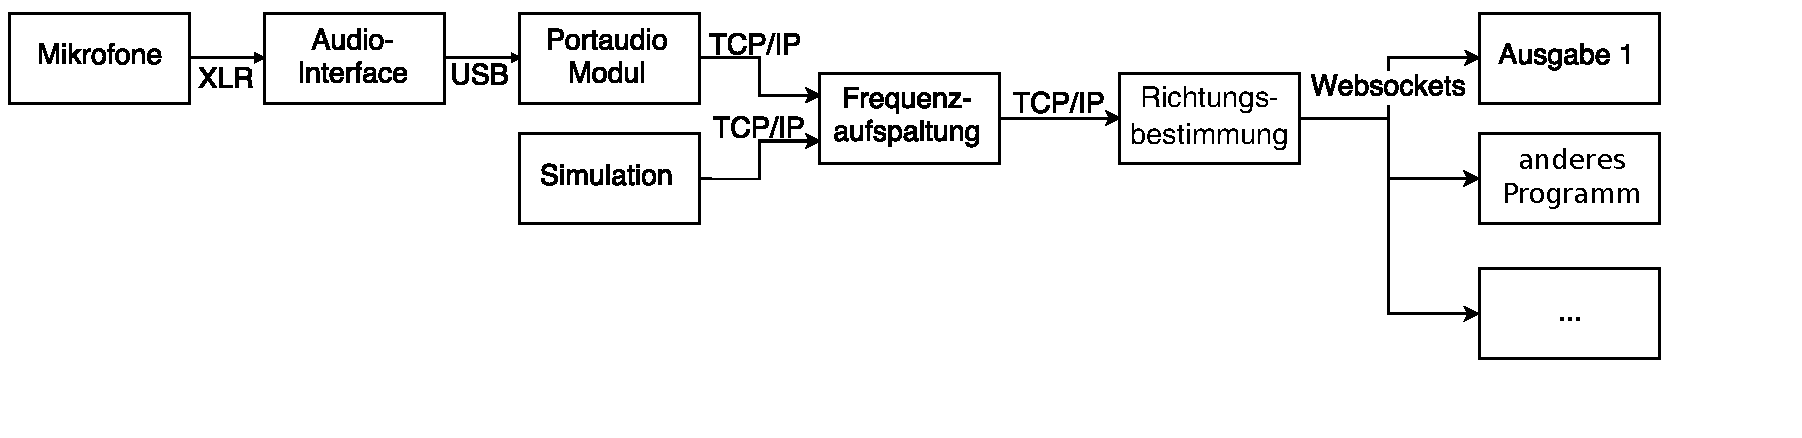
\includegraphics[width=\linewidth]{img/flowchart}
	\caption{Der modulare Aufbau unseres Konzeptes}
	\label{fig:flowchart}
\end{figure}

\subsection{Audiosimulation (Modul 1)}
Um die Richtungsbestimmung unabhängig von Störfaktoren wie dem Rauschen und der Reflexion des Schalls an Wänden oder anderen Gegenständen zu überprüfen, haben wir zunächst eine Simulation entwickelt. Außerdem lässt sich mit dieser gezielt der Einfluss verschiedener Störfaktoren untersuchen. Die Simulation kann beliebig viele Mikrofone an beliebigen Positionen simulieren. Leider konnten wir keine bestehenden Lösungen für die Simulation von dreidimensionalem Ton, wie \textit{OpenAL} \cite{OpenAL}, welches eine Programmbibliothek für die Simulation von Schall ist, verwenden, da bei diesen die Anzahl der Mikrofone limitiert ist und die Phase des Audiosignals in der Simulation vernachlässigt wird. Da die Funktion unserer Richtungsbestimmung unabhängig von den Amplituden der Schallquellen bei den einzelnen Mikrofonen ist, haben wir unsere Simulation rein auf die Phase und die Laufzeit beschränkt. Um eine interaktive Benutzung und eine leichte Überprüfung der Richtungsbestimmung zu gewährleisten, besitzt die Simulation eine graphische Benutzeroberfläche, mit der man interaktiv Schallquellen hinzufügen und entfernen kann. Außerdem kann die Simulation auch die bestimmten Richtungen darstellen und ermöglicht damit einen einfachen Vergleich der bestimmten und tatsächlichen Richtungen. Das Simulationsmodul wurde in der Programmiersprache \textit{C++} implementiert, da diese eine gute \textit{OpenGL} Integration bietet.

\begin{figure}[H]
	\centering
  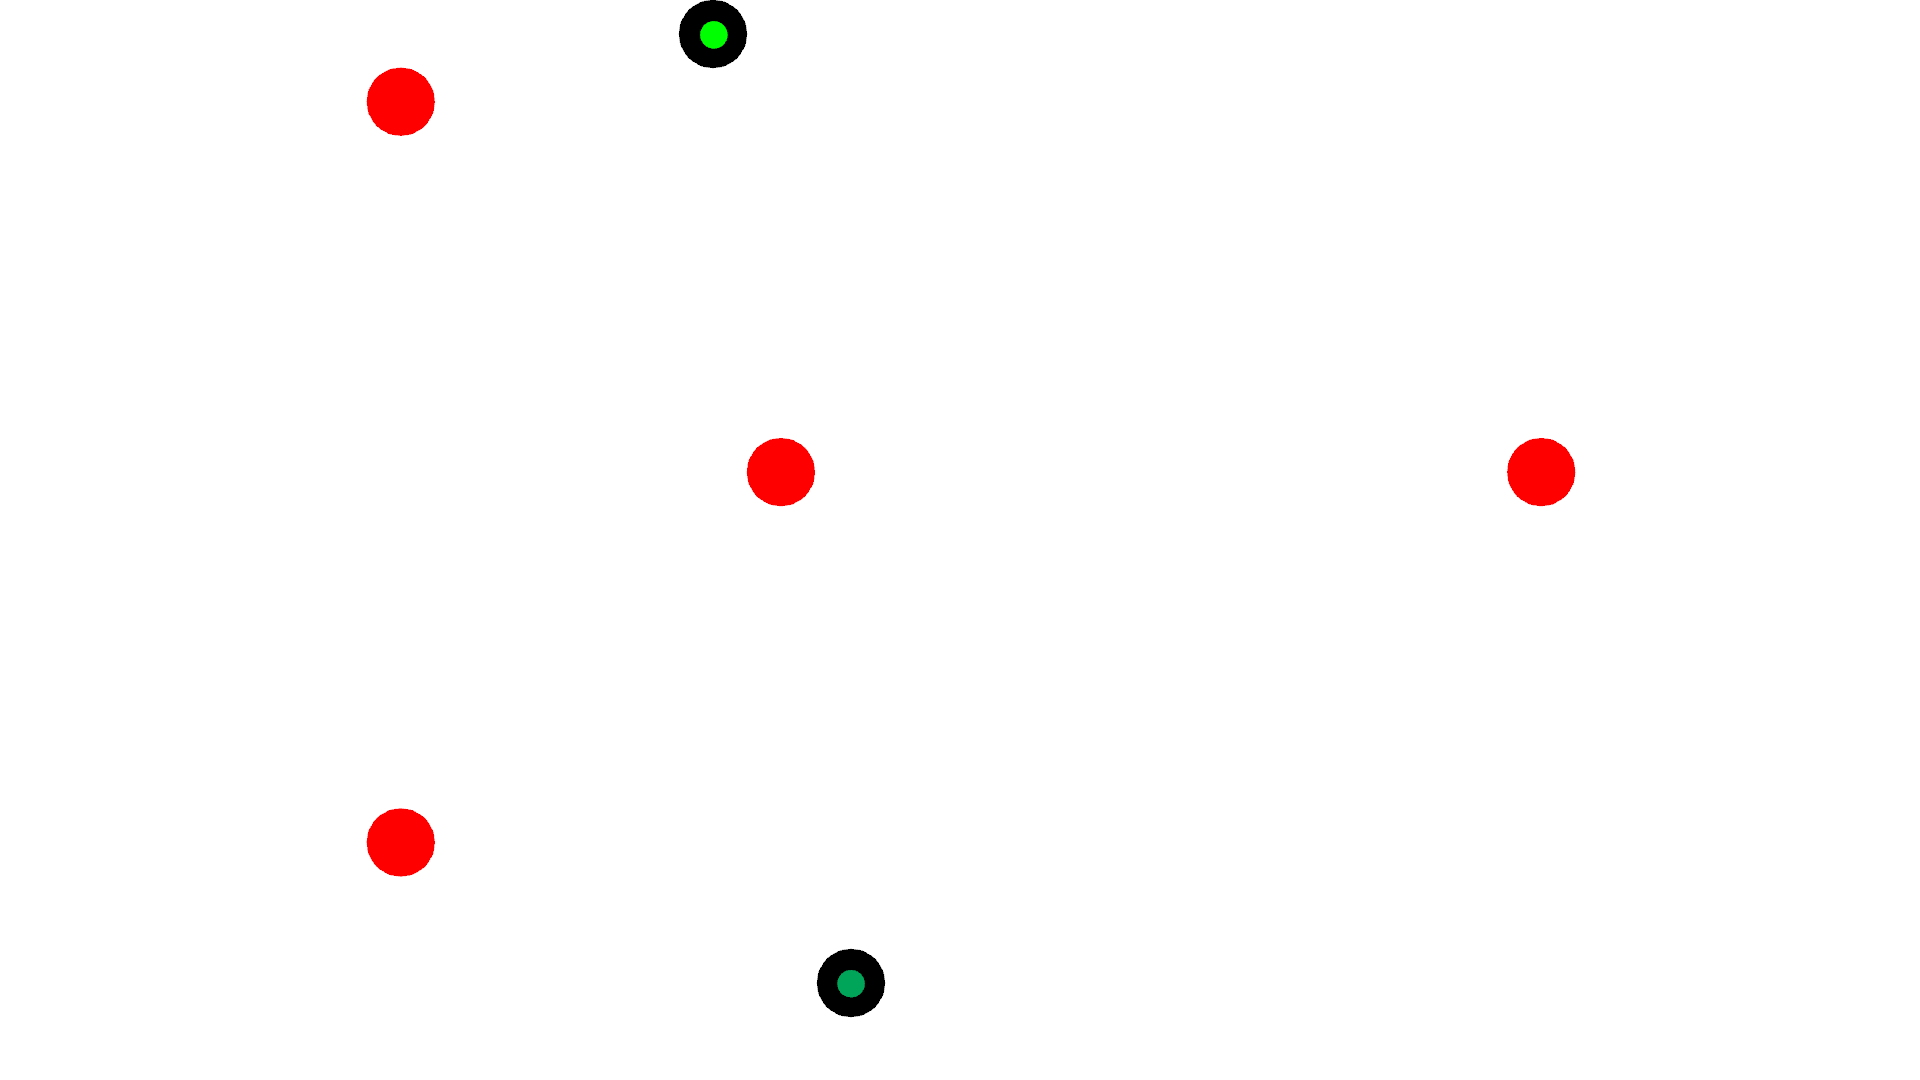
\includegraphics[width=(0.7\linewidth)]{img/bildsimulation}
  \caption{Screenshot der Simulation, die roten Punkte stellen die Mikrofone dar, die schwarzen die Schallquellen und die grünen die georteten Positionen}
\end{figure}

\subsection{Hardware (Modul 1)}
\begin{wrapfigure}{R}{0.4\textwidth}
	\centering
	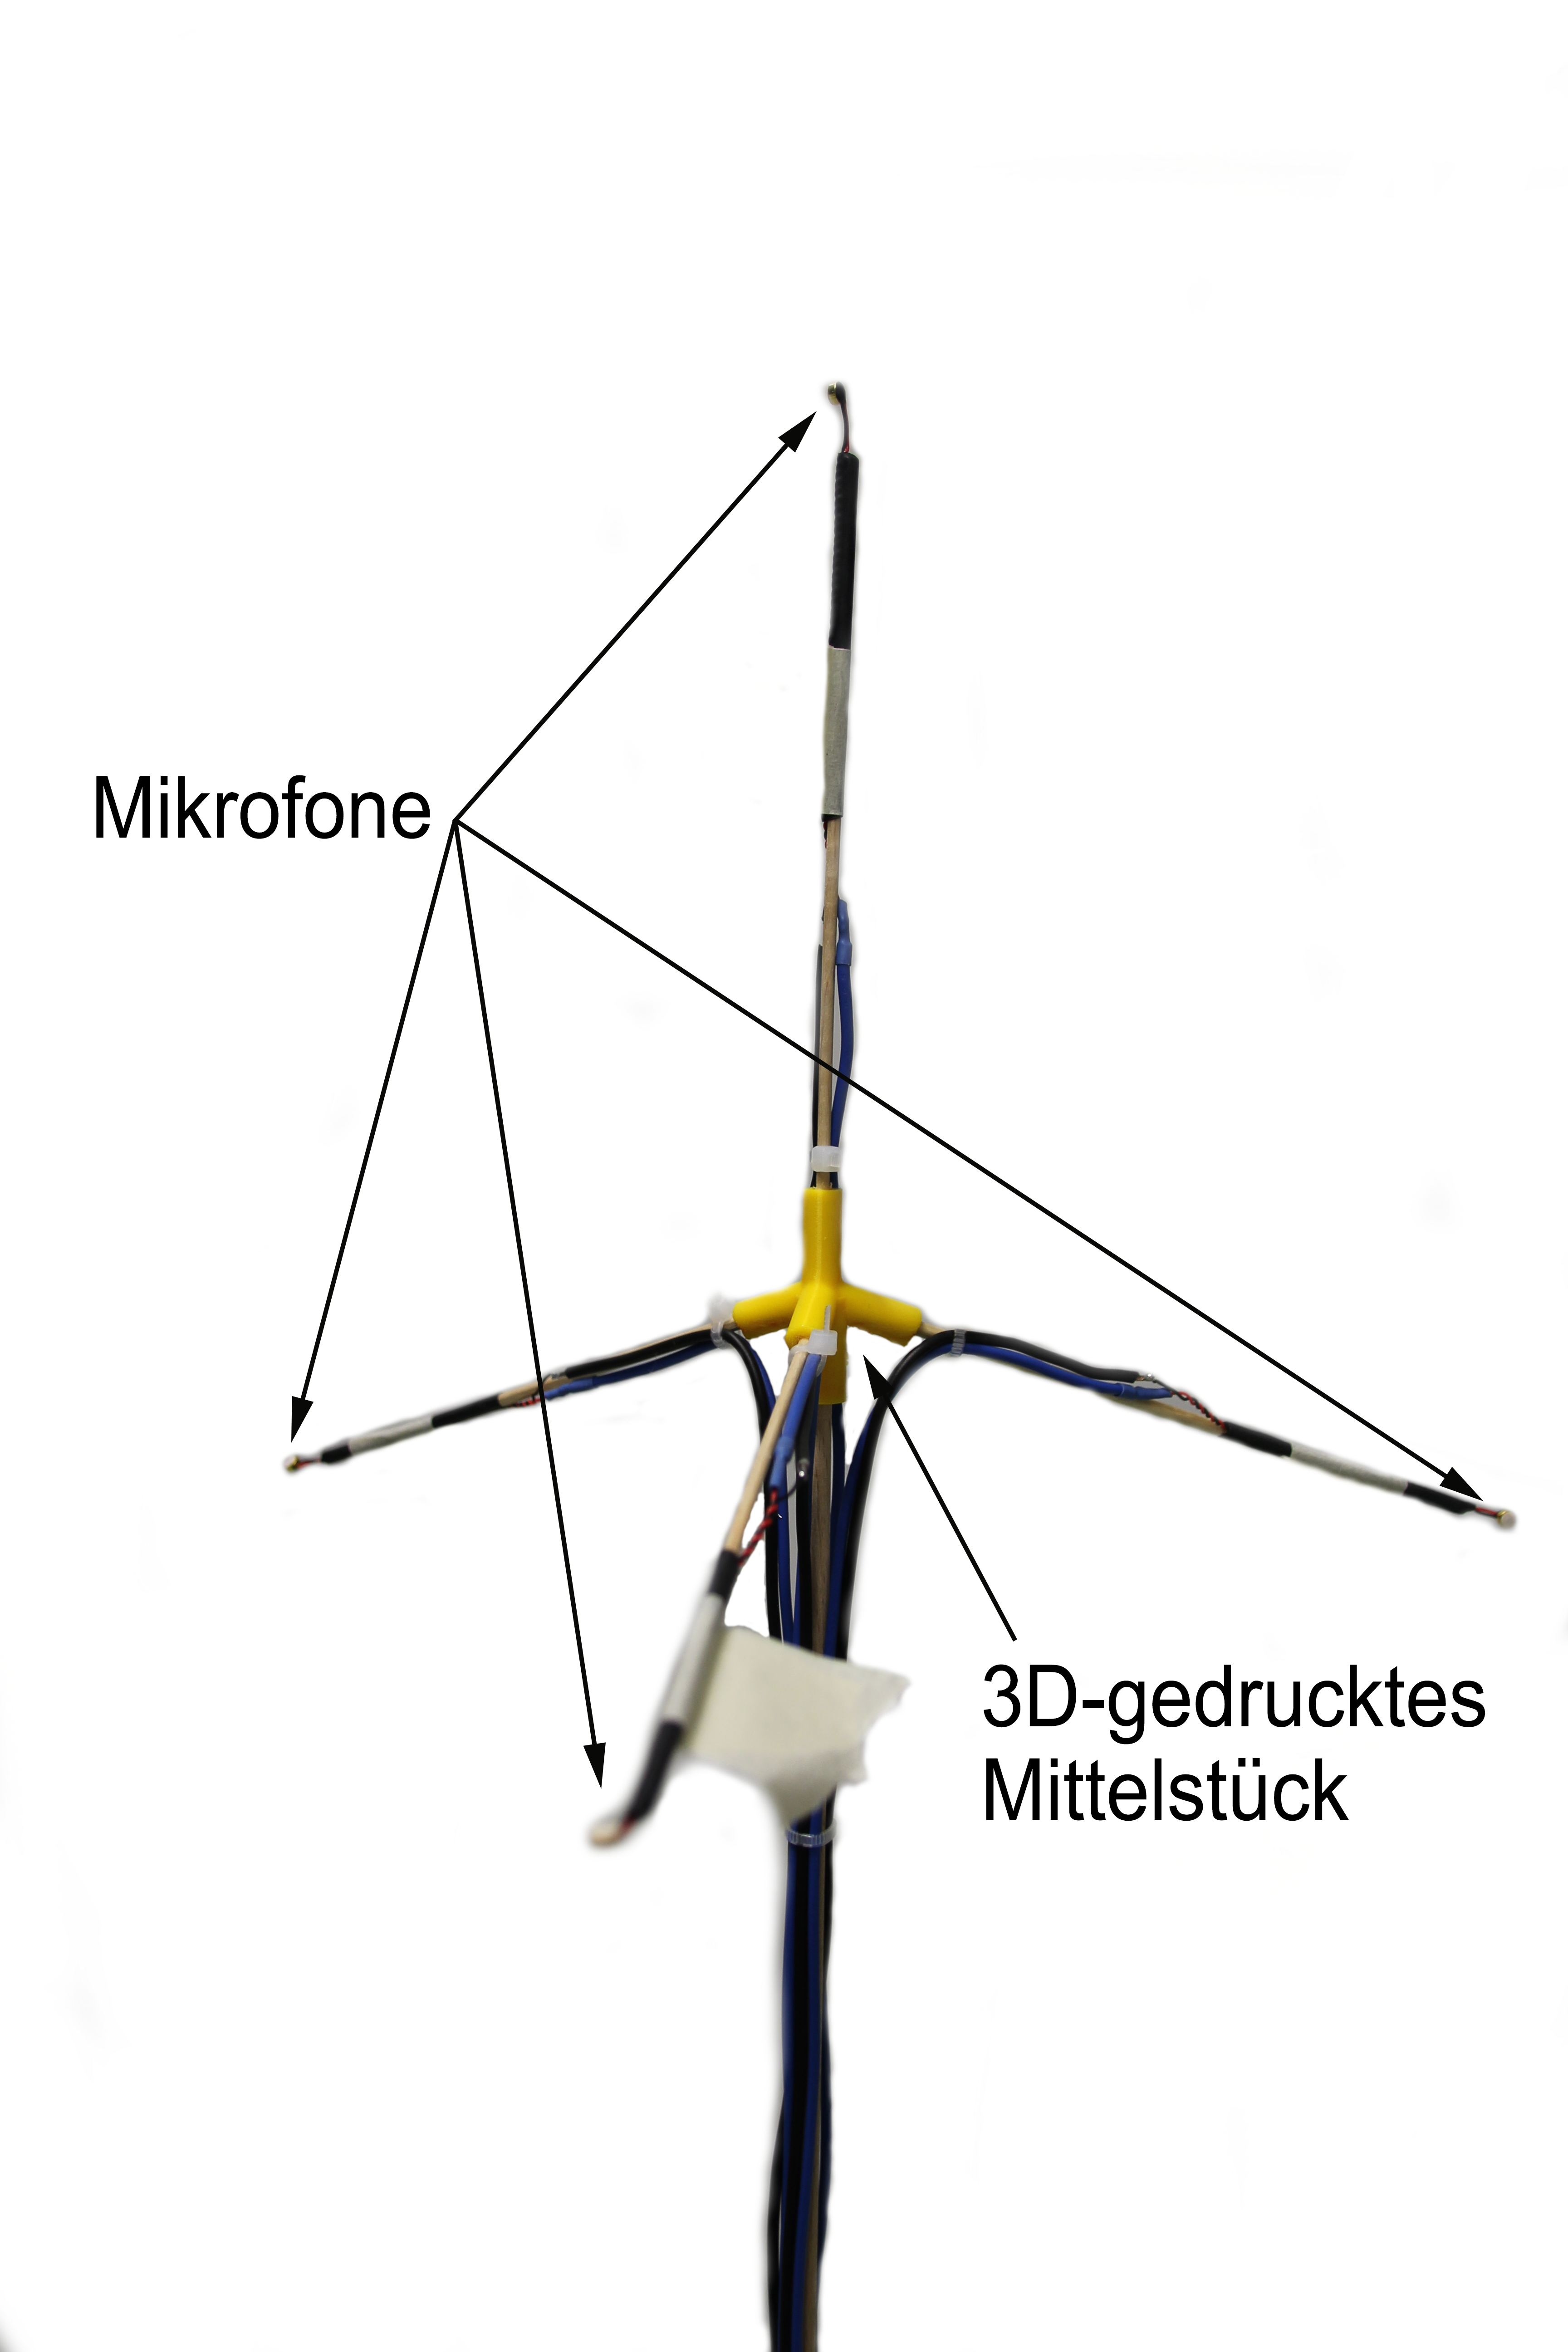
\includegraphics[width=\linewidth]{img/tet}
	\caption{Aufbau unserer Messapparatur}
\end{wrapfigure}
Um das durch die Simulation evaluierbare Verfahren praktisch zu testen und zu nutzen, muss nur die Quelle der Daten, also das erste Modul, ausgetauscht werden. Die Aufgabe des ersten Moduls ist es nun nicht mehr, virtuelle Mikrofone, welche die Aufnahme von virtuellen Schallquellen simulieren zu produzieren, sondern die Signale echter Mikrofone, welche echte Schallquellen aufnehmen, einzulesen. Um die Signale der Mikrofone mit einem Computer zu verarbeiten müssen sie digitalisiert werden. Zusätzlich benötigt man eine alternative Implementation der des ersten Moduls, die die Daten von der Hardware annimmt und an das zweite Modul weiterleitet. Hierbei kommen wieder die Vorteile unserer modularen Vorgehensweise zum tragen, da nur das erste Modul ersetzt werden muss und die gesamte restliche Software beibehalten werden kann. Dies sorgt auch dafür, dass die Simulation und die Realwelttests immer die gleichen Auswertungsalgorithmen verwenden und so sehr gut vergleichbar sind.
\subsubsection{Mikrofone}
Die erste Komponente, die es bei einem realen Aufbau der Messapparatur eine wichtige Rolle spielt, ist die der Schallwandlung. Dies wird durch Mikrofone realisiert, an die es einige Anforderungen gibt. Die wichtigste Anforderung ist, dass sie eine möglichst gleichmäßige Richtcharakteristik haben.
Eine weitere Anforderung ist, dass sie möglichst klein sind, da der Abstand zwischen ihnen nicht zu groß sein darf, um die obere Grenzfrequenz möglichst hoch zu setzen, da der Abstand der Mikrofone nicht größer als die Wellenlänge der zu lokalisierenden Frequenz sein darf. Des weiteren sollte das Signal-Rausch-Verhältnis möglichst groß sein, da Rauschen die Messungen unpräziser macht \cite{Rausch}.
Wir haben uns dafür entschieden, Elektretmikrofonkapseln zu verwenden, da diese üblich sind, keine aufwendige Elektronik zur Ansteuerung benötigen und die oben aufgeführten Anforderungen relativ gut erfüllen \cite{elektret}.
Die meisten für uns relevanten Parameter der Mikrofone konnten wir aus den Datenblättern entnehmen. Eine Ausnahme hiervon ist die Richtcharakteristik, welche jedoch für uns sehr wichtig ist, da sie die Messqualität sehr stark beeinflusst. Diese sollte möglichst gleichmäßig sein, da nur so aus allen Richtungen Daten von gleicher Qualität aufgenommen werden können. Wenn zum Beispiel alle Mikrofone eine Nierencharakteristik aufweisen und sie in einem gleichseitigen Dreieck angeordnet sind, liefert mindestens ein Mikrofon ein deutlich schwächeres Signal als die anderen, was dazu führt, das die Phasenlage der einzelnen Wellen ungenauer bestimmt werden und mit ihnen auch die Lokalisation ungenauer wird.
Um unter diesem Aspekt geeignete Mikrofone zu finden, haben wir die Richtcharakteristiken verschiedener Mikrofone mittels einer selbst entwickelten Messapparatur und einer selbst entwickelten Messsoftware vermessen. Die hierfür entwickelte Messapparatur sendet mittels eines Lautsprechers eine Sinus-Schwingung aus und misst, wie stark diese vom Mikrofon aufgenommen wurde. Danach dreht sie das Mikrofon um einen festgelegten Winkel weiter und fertigt erneut eine Messung an. Dieser Vorgang wird solange wiederholt, bis das Mikrofon einmal um 360$^{\circ}$ gedreht wurde.
\begin{figure}[H]
  \centering
  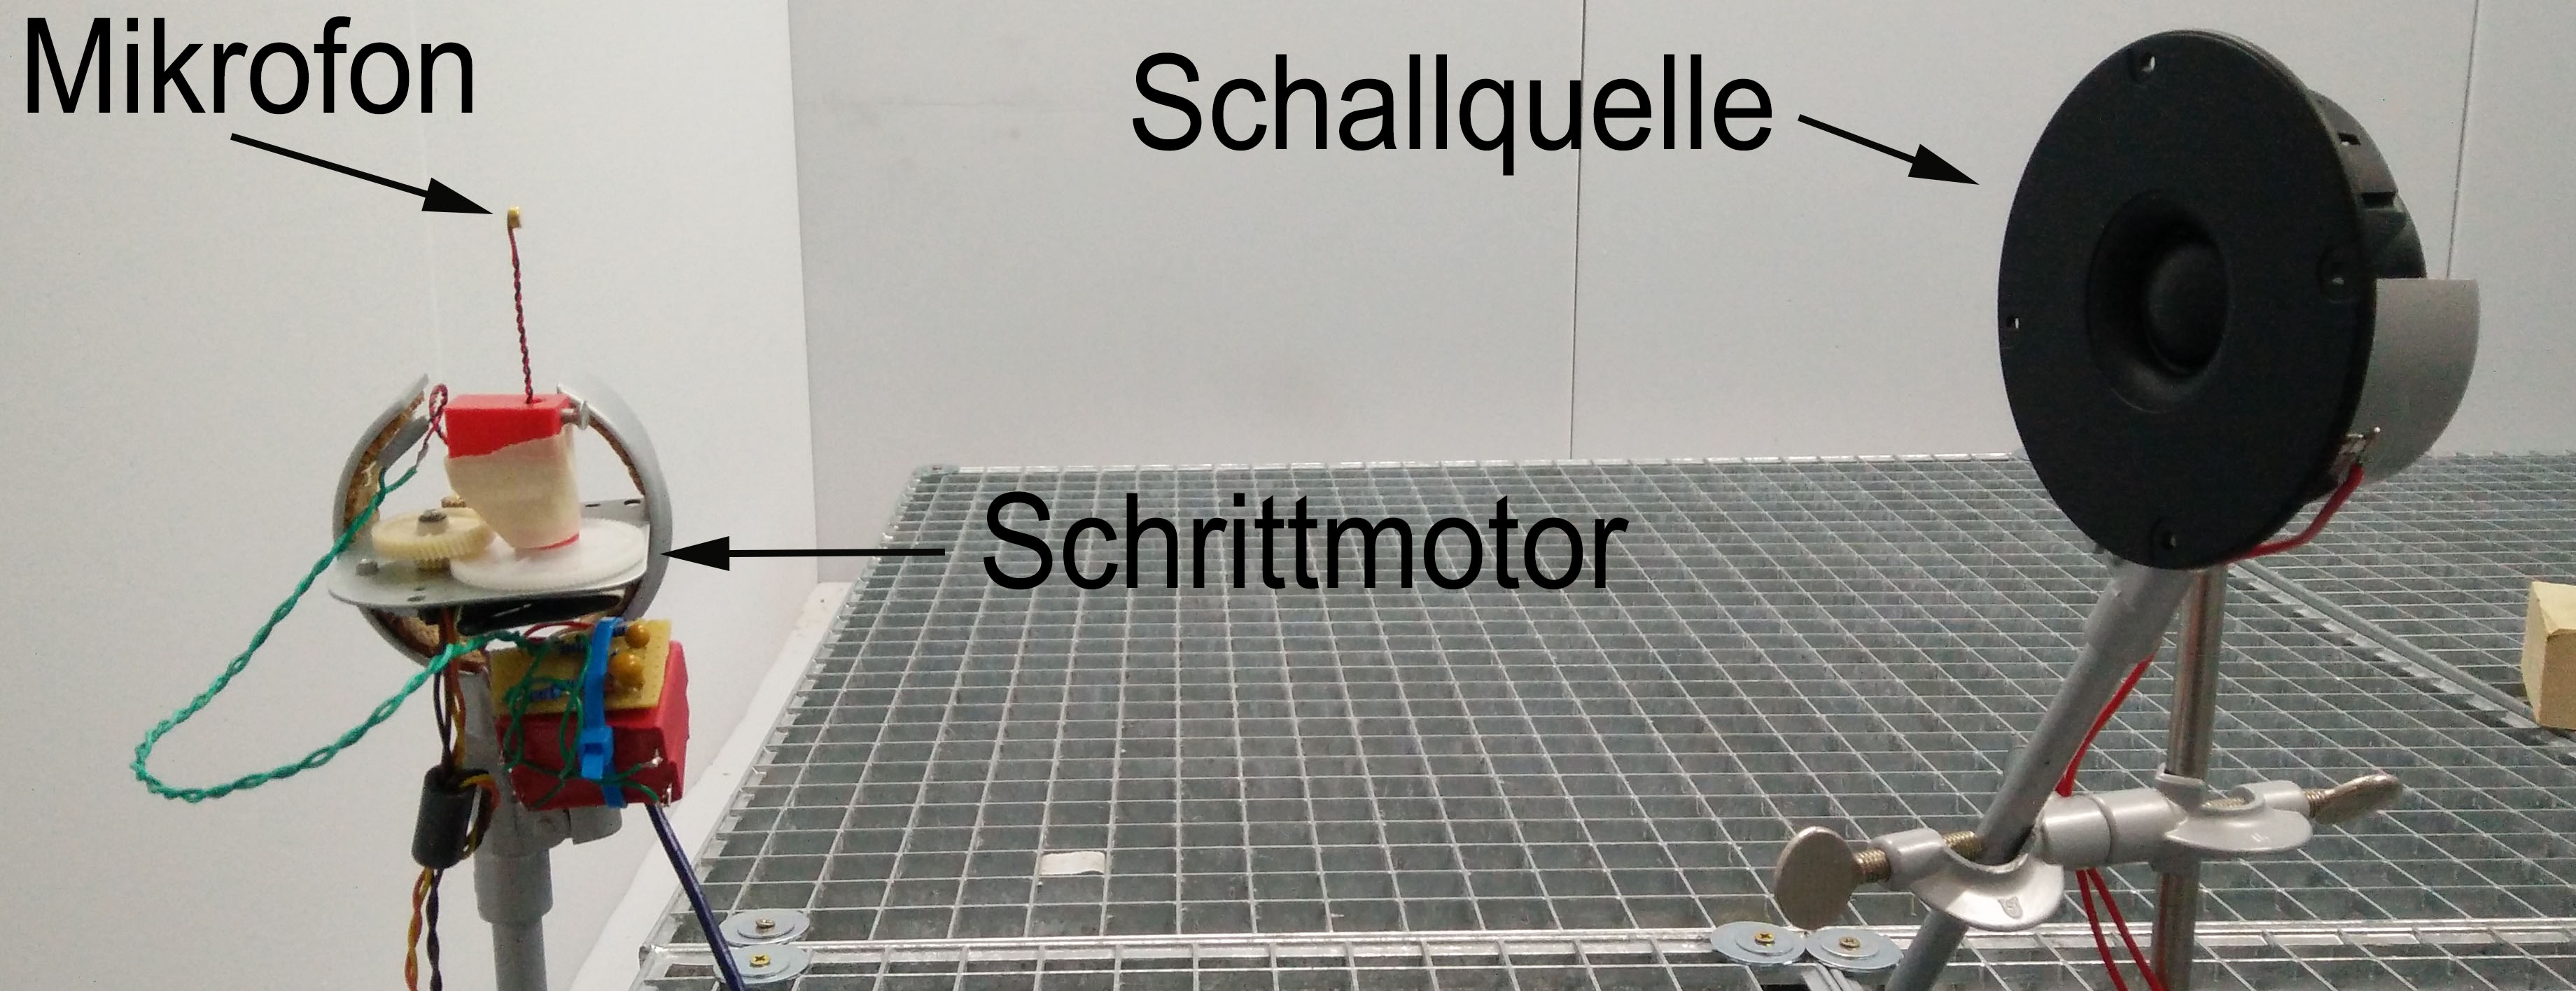
\includegraphics[width=0.8\linewidth]{img/chara_mess}
  \caption{Unsere Messapparatur für die Charakteristik eines Mikrofons}
\end{figure}
Die so ermittelten Daten können nun mittels des freien Plottingprogramms \textit{gnuplot}~\cite{Gnuplot} visualisiert werden, um die Richtcharakteristik abzulesen.
\begin{figure}[H]
  \centering
  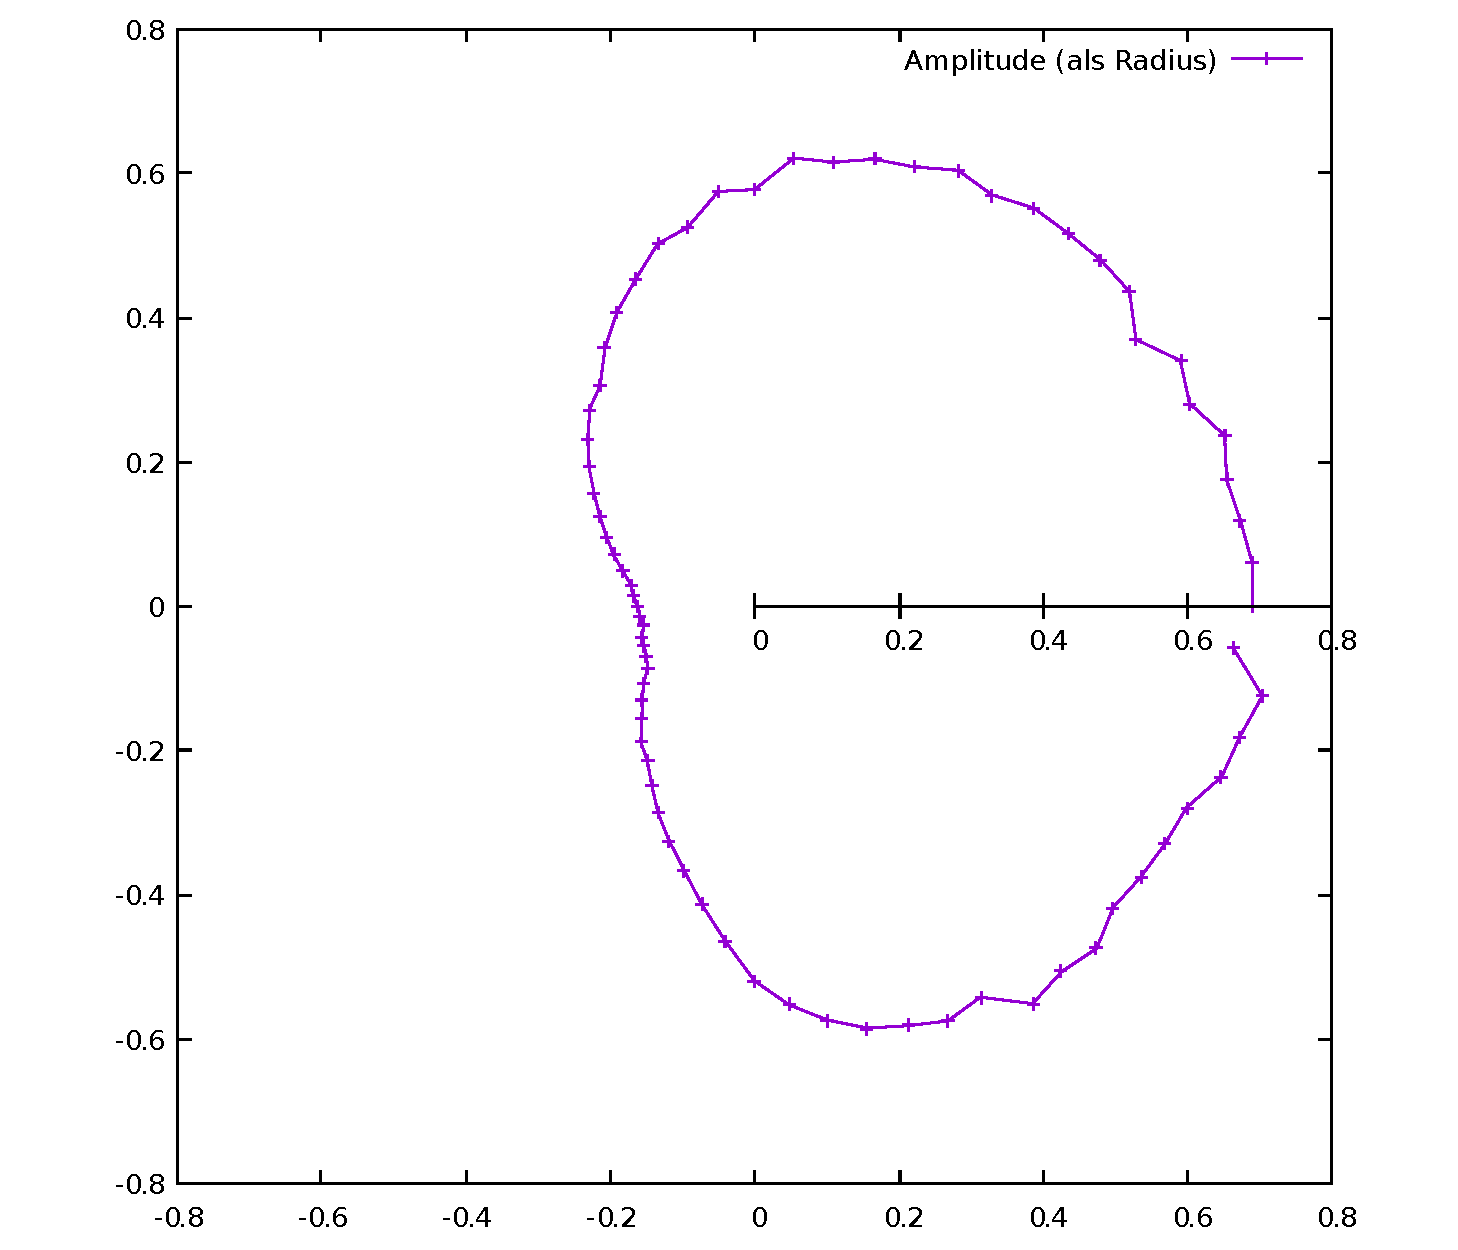
\includegraphics[width=0.45\linewidth]{img/badMic}
  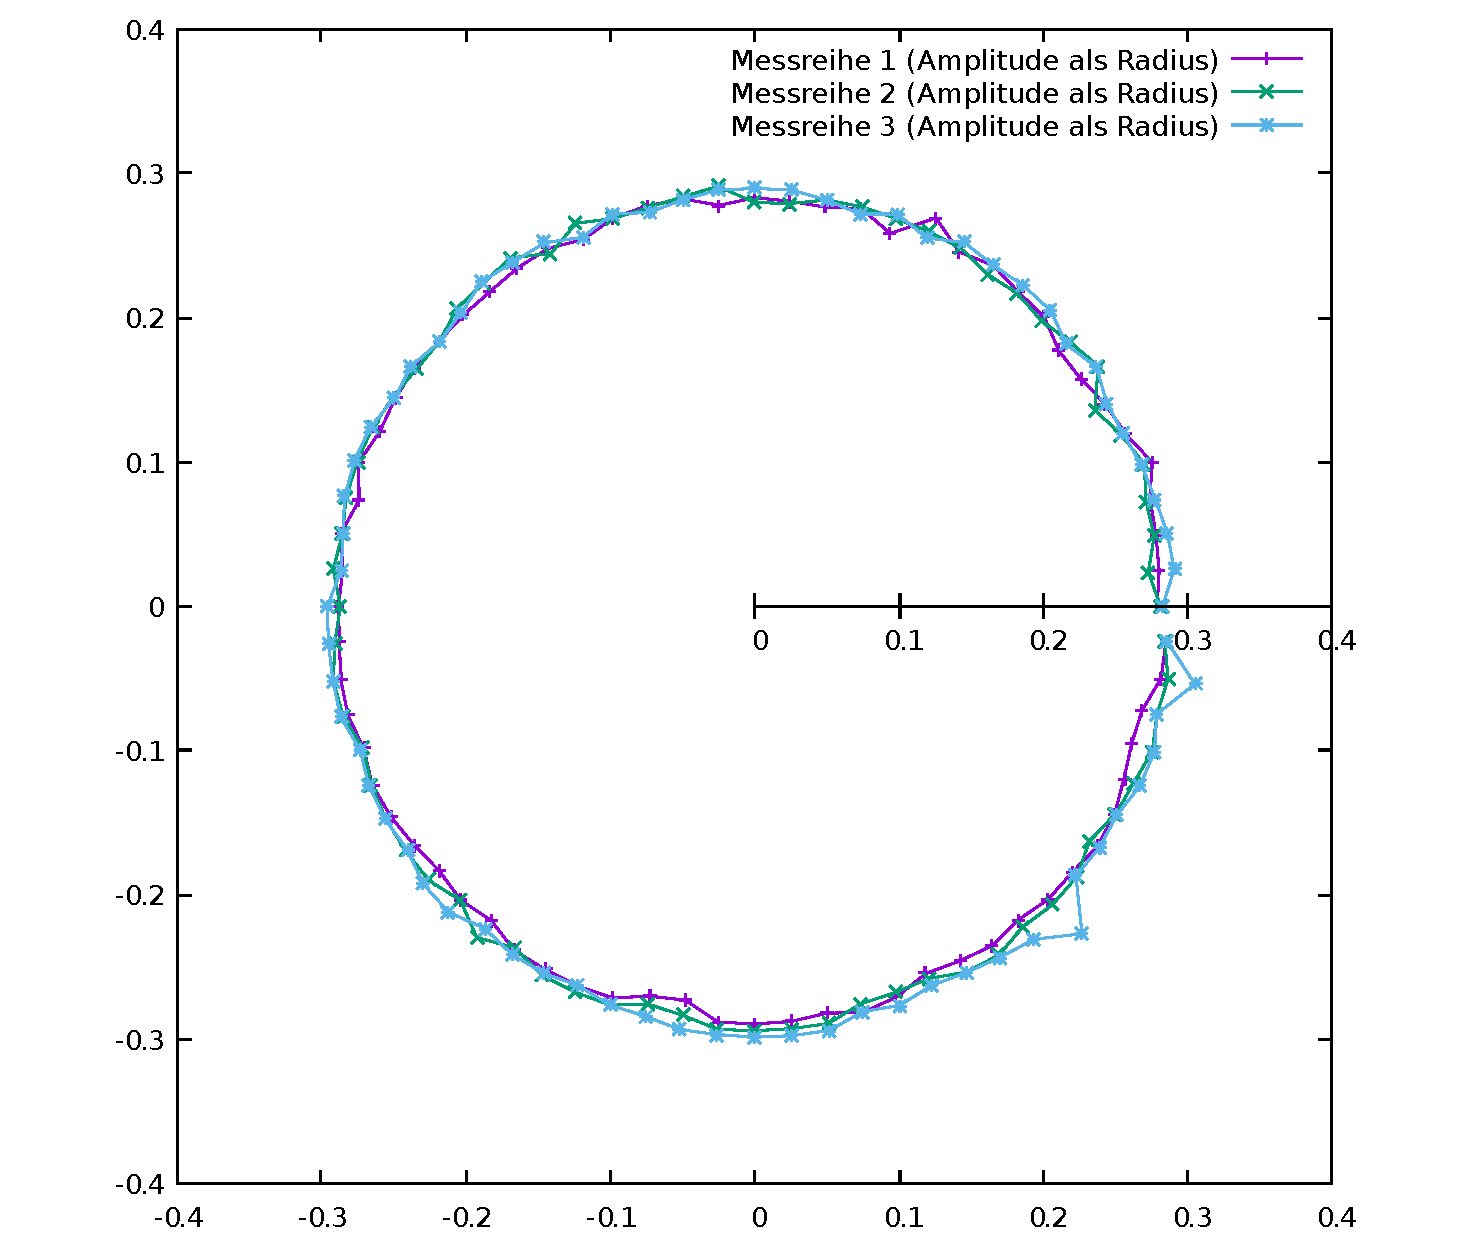
\includegraphics[width=0.45\linewidth]{img/goodMic}
  \caption{Auf den beiden Grafiken ist die gemessene Amplitude des Mikrofons über den Winkel aufgetragen. Bei der linken Grafik kann man feststellen, dass das vermessene Mikrofon eine sehr ungleichmäßige Charakteristik aufweist, diese Mikrofone haben wir zu Anfang verwendet. Auf der rechten Seite ist die Charakteristik der Mikrofone zu sehen, die wir in unserem aktuellen Testaufbau verwenden. Diese ist sehr gleichmäßig, weshalb wir die zuerst verwendeten Mikrofone durch diese Mikrofone ausgetauscht haben.}\label{fig:caracter}
\end{figure}
Für die reale Messapparatur haben wir vier Mikrofone in einem Tetraeder angeordnet. Dadurch, dass ein Tetraeder symmetrisch ist, sind die Fehler in alle Richtungen ungefähr gleich groß und die Richtungsbestimmung ist in allen Richtungen gleich gut. Um die Charakteristik der Mikrofone möglichst wenig zu verändern, haben wir die Mikrofone nur an ihrem Kabel mit dem Tetraeder verbunden. Dadurch ist der Schallschatten durch den Tetraeder relativ gering. Das Mittelstück des Tetraeders haben wir mit Hilfe eines 3D Druckers hergestellt.
\subsubsection{Audiointerface}
Auch an das Audiointerface, also die Verbindung von Mikrofonen zum Computer, gibt es bestimmte Voraussetzungen. So benötigt unser Verfahren mindestens 4 Mikrofone, jedoch lässt es sich einfach auf mehr Kanäle erweitern, was der Genauigkeit zugute kommt. Daher wird ein Audiointerface mit möglichst vielen Kanälen gesucht. Eine weitere wichtige Anforderung an das Audiointerface ist eine hohe Auflösung, da hierdurch die Signalqualität verbessert wird und digitale Verstärkung bei ausreichender Audioqualität möglich ist. Um die Elekretmikrofonkapseln an das Audiointerface anzuschließen, benötigt man zusätzlich eine Schaltung, welche das unsymmetrische Signal der Elektretmikrofonkapsel in ein symmetrisches Signal für das Audiointerface umwandelt. Außerdem muss diese die Phantomspeisung, die das Audiointerface bereitstellt und eine Spannung von 48V hat, in eine Tonaderspeisung für das Mikrofon konvertieren. Hierfür kommt die Schaltung von \cite{Powering_microphones} zum Einsatz.

\subsubsection{Software}
Um die echten Mikrofone für die Richtungsbestimmung zu verwenden, muss noch eine Verbindung zwischen dem Audiointerface und dem nächsten Modul geschaffen werden. Durch unseren modularen Aufbau lässt sich dies leicht implementieren. Wir haben dazu ein Programm in Java entwickelt, dass fähig ist, mehrkanalige Audiosignale in Echtzeit aufzunehmen und über TCP/IP an die Fourier-Transformation weiterzuleiten. Zur Umsetzung haben wir die Programmbibliothek \textit{portaudio} \cite{portaudio} verwendet. Diese Programmbibliothek hat den Vorteil, dass mehrere Audiokanäle zeitsynchronisiert eingelesen werden können, was sehr wichtig ist, damit unser Verfahren zur Richtungsbestimmung, welches auf der relativen Phasenlage basiert, funktioniert. \textit{Portaudio} wurde unter Java über das Java Native Interface (JNI) benutzt.

\subsection{Fourier-Transformation (Modul 2)}
Dieses Modul teilt die Audio-Signale in einzelnen Sinuswellen und bestimmt deren Phase und Amplitude. Um dies zu bewerkstelligen, lässt sich eine diskrete Fourier-Transformation verwenden. Die diskrete Fourier-Transformation bestimmt aus einem zeitdiskretem Signal die einzelnen Sinusschwingungen mit ihrer zugehörigen Phase und Amplitude, die zusammen das Signal bilden. Ein schneller Algorithmus um die diskrete Fourier-Transformation eines Signals zu berechnen ist die Fast Fourier-Transformation (FFT). Dieser ist schnell genug, um eine Echtzeitverarbeitung des Signals zu ermöglichen. Als Implementation der FFT haben wir \textit{FFTW}\cite{FFTW} verwendet, da \textit{FFTW} kostenlos, opensource und vergleichsweise schnell ist.
Das Fourier-Transformations Modul wurde aus Performancegründen in \textit{C++} implementiert.
Aus einer diskreten Fourier-Transformation von $n$ reellen Zahlen erhält man eine Liste aus $n$ komplexen Zahlen. Eine komplexe Zahl $z$ an der Stelle $i$ enthält die Amplituden- und Phaseninformation für die Frequenz $f$:
$$
f = \frac{i\cdot r}{n}
$$
$r$ ist dabei die Abtastrate des Signals. Die Amplitude $A$ des Sinus lässt sich mit dem Betrag der komplexen Zahl berechnen und die Phase $\phi$ mit dem Arcus-Tangens, dies entspricht der Koordinatentransformation von einem kartesischem in das polare Koordinatensystem:\\
\begin{minipage}{0.49\textwidth}
  $$
  A = \sqrt[]{{\Re(z)}^2 + {\Im(z)}^2}
  $$
  $$
  \phi = \operatorname{atan2}(\Im(z), \Re(z))
  $$
  $$
  \operatorname{atan2}(y,x) := \begin{cases} \arctan\frac{y}{x} & \mathrm{f\ddot ur}\ x > 0\\ \arctan\frac{y}{x} + \pi & \mathrm{f\ddot ur}\ x < 0,\ y \geq 0\\ \arctan\frac{y}{x} - \pi & \mathrm{f\ddot ur}\ x < 0,\ y < 0\\ +\pi/2 & \mathrm{f\ddot ur}\ x = 0,\ y > 0\\ -\pi/2 & \mathrm{f\ddot ur}\ x = 0,\ y < 0\\ 0 & \mathrm{f\ddot ur}\ x = 0,\ y = 0 \end{cases}
  $$
\end{minipage}
\begin{minipage}{0.49\textwidth}
  \begin{figure}[H]
    \centering
    \scalebox{.7}{% GNUPLOT: LaTeX picture with Postscript
\begingroup
  \fontfamily{phv}%
  \selectfont
\definecolor{t}{rgb}{0.5,0.5,0.5}
  \makeatletter
  \providecommand\color[2][]{%
    \GenericError{(gnuplot) \space\space\space\@spaces}{%
      Package color not loaded in conjunction with
      terminal option `colourtext'%
    }{See the gnuplot documentation for explanation.%
    }{Either use 'blacktext' in gnuplot or load the package
      color.sty in LaTeX.}%
    \renewcommand\color[2][]{}%
  }%
  \providecommand\includegraphics[2][]{%
    \GenericError{(gnuplot) \space\space\space\@spaces}{%
      Package graphicx or graphics not loaded%
    }{See the gnuplot documentation for explanation.%
    }{The gnuplot epslatex terminal needs graphicx.sty or graphics.sty.}%
    \renewcommand\includegraphics[2][]{}%
  }%
  \providecommand\rotatebox[2]{#2}%
  \@ifundefined{ifGPcolor}{%
    \newif\ifGPcolor
    \GPcolortrue
  }{}%
  \@ifundefined{ifGPblacktext}{%
    \newif\ifGPblacktext
    \GPblacktextfalse
  }{}%
  % define a \g@addto@macro without @ in the name:
  \let\gplgaddtomacro\g@addto@macro
  % define empty templates for all commands taking text:
  \gdef\gplbacktext{}%
  \gdef\gplfronttext{}%
  \makeatother
  \ifGPblacktext
    % no textcolor at all
    \def\colorrgb#1{}%
    \def\colorgray#1{}%
  \else
    % gray or color?
    \ifGPcolor
      \def\colorrgb#1{\color[rgb]{#1}}%
      \def\colorgray#1{\color[gray]{#1}}%
      \expandafter\def\csname LTw\endcsname{\color{white}}%
      \expandafter\def\csname LTb\endcsname{\color{black}}%
      \expandafter\def\csname LTa\endcsname{\color{black}}%
      \expandafter\def\csname LT0\endcsname{\color[rgb]{1,0,0}}%
      \expandafter\def\csname LT1\endcsname{\color[rgb]{0,1,0}}%
      \expandafter\def\csname LT2\endcsname{\color[rgb]{0,0,1}}%
      \expandafter\def\csname LT3\endcsname{\color[rgb]{1,0,1}}%
      \expandafter\def\csname LT4\endcsname{\color[rgb]{0,1,1}}%
      \expandafter\def\csname LT5\endcsname{\color[rgb]{1,1,0}}%
      \expandafter\def\csname LT6\endcsname{\color[rgb]{0,0,0}}%
      \expandafter\def\csname LT7\endcsname{\color[rgb]{1,0.3,0}}%
      \expandafter\def\csname LT8\endcsname{\color[rgb]{0.5,0.5,0.5}}%
    \else
      % gray
      \def\colorrgb#1{\color{black}}%
      \def\colorgray#1{\color[gray]{#1}}%
      \expandafter\def\csname LTw\endcsname{\color{white}}%
      \expandafter\def\csname LTb\endcsname{\color{black}}%
      \expandafter\def\csname LTa\endcsname{\color{black}}%
      \expandafter\def\csname LT0\endcsname{\color{black}}%
      \expandafter\def\csname LT1\endcsname{\color{black}}%
      \expandafter\def\csname LT2\endcsname{\color{black}}%
      \expandafter\def\csname LT3\endcsname{\color{black}}%
      \expandafter\def\csname LT4\endcsname{\color{black}}%
      \expandafter\def\csname LT5\endcsname{\color{black}}%
      \expandafter\def\csname LT6\endcsname{\color{black}}%
      \expandafter\def\csname LT7\endcsname{\color{black}}%
      \expandafter\def\csname LT8\endcsname{\color{black}}%
    \fi
  \fi
    \setlength{\unitlength}{0.0500bp}%
    \ifx\gptboxheight\undefined%
      \newlength{\gptboxheight}%
      \newlength{\gptboxwidth}%
      \newsavebox{\gptboxtext}%
    \fi%
    \setlength{\fboxrule}{0.5pt}%
    \setlength{\fboxsep}{1pt}%
\begin{picture}(5896.00,3600.00)%
    \gplgaddtomacro\gplbacktext{%
      \colorrgb{0.50,0.50,0.50}%
      \put(990,576){\makebox(0,0)[r]{\strut{}\color{t}$-1$}}%
      \colorrgb{0.50,0.50,0.50}%
      \put(990,1278){\makebox(0,0)[r]{\strut{}\color{t}$-0.5$}}%
      \colorrgb{0.50,0.50,0.50}%
      \put(990,1980){\makebox(0,0)[r]{\strut{}\color{t}$0$}}%
      \colorrgb{0.50,0.50,0.50}%
      \put(990,2681){\makebox(0,0)[r]{\strut{}\color{t}$0.5$}}%
      \colorrgb{0.50,0.50,0.50}%
      \put(990,3383){\makebox(0,0)[r]{\strut{}\color{t}$1$}}%
      \colorrgb{0.50,0.50,0.50}%
      \put(1098,396){\makebox(0,0){\strut{}\color{t}$-1$}}%
      \colorrgb{0.50,0.50,0.50}%
      \put(2216,396){\makebox(0,0){\strut{}\color{t}$-0.5$}}%
      \colorrgb{0.50,0.50,0.50}%
      \put(3335,396){\makebox(0,0){\strut{}\color{t}$0$}}%
      \colorrgb{0.50,0.50,0.50}%
      \put(4453,396){\makebox(0,0){\strut{}\color{t}$0.5$}}%
      \colorrgb{0.50,0.50,0.50}%
      \put(5571,396){\makebox(0,0){\strut{}\color{t}$1$}}%
      \csname LTb\endcsname%
      \put(3178,2050){\makebox(0,0)[l]{\strut{}$\phi$}}%
      \put(4341,1442){\makebox(0,0)[l]{\strut{}$A$}}%
    }%
    \gplgaddtomacro\gplfronttext{%
      \csname LTb\endcsname%
      \put(144,1979){\rotatebox{-270}{\makebox(0,0){\strut{}Imaginärteil}}}%
      \put(3334,126){\makebox(0,0){\strut{}Realteil}}%
      \csname LTb\endcsname%
      \put(4752,3230){\makebox(0,0)[r]{\strut{}z}}%
    }%
    \gplbacktext
    \put(0,0){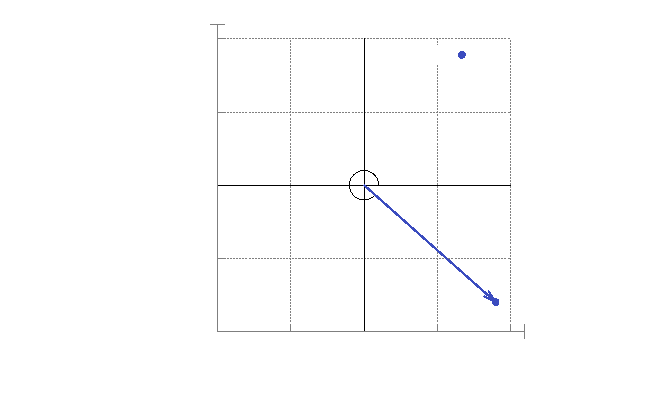
\includegraphics{img/polarconvert}}%
    \gplfronttext
  \end{picture}%
\endgroup
}
    \caption{Transformation von kartesischen zu polaren Koordinatensystem}
    \label{fig:polarconvert}
  \end{figure}
\end{minipage}
\vspace{20pt}
\\
Die Verwendung von $\operatorname{atan2}(y,x)$ anstelle von $\arctan\frac{y}{x}$ sorgt dafür, dass der richtige Winkel berechnet wird. $\arctan\frac{y}{x}$ liefert nur Winkel von -90\degree bis 90\degree, deswegen muss anhand des Vorzeichens von $x$ und $y$ bestimmt werden, in welchem Quadranten der Punkt liegt und der von $\arctan\frac{y}{x}$ gelieferte Winkel dementsprechend verschoben werden.

Das in Frequenz, Phase und Amplitude konvertierte Ergebnis der Fourier-Transformation wird dann gefiltert. Alle Frequenzen mit einer Amplitude, die kleiner als eine bestimmte Untergrenze ist, werden verworfen. Die verbleibenden Frequenzen werden an das Richtungsmodul übermittelt.

\subsection{Richtungsmodul (Modul 3)}
Die von der Fourier-Transformation bestimmten Tripel aus Frequenz, Phase und Amplitude werden vom Richtungsmodul weiter verarbeitet. In das Richtungsmodul können verschiedene Methoden der Richtungsbestimmung eingesetzt werden. Das Verfahren zur Richtungsbestimmung, das von dem Richtungsmodul verwendet wird, kann einfach ausgetauscht werden. Die ermittelten Richtungen werden an die Ausgabe weitergesendet um sie dort auszugeben oder zur Filterung des Audio-Signals zu verwenden.
Das Richtungsmodul ist in C++ geschrieben und verwendet \textit{LAPACK}\cite{Anderson:1990:LPL:110382.110385}.
\subsection{Ausgabemodul (Modul 4)}
\begin{wrapfigure}{r}{0.5\textwidth}
	\centering
	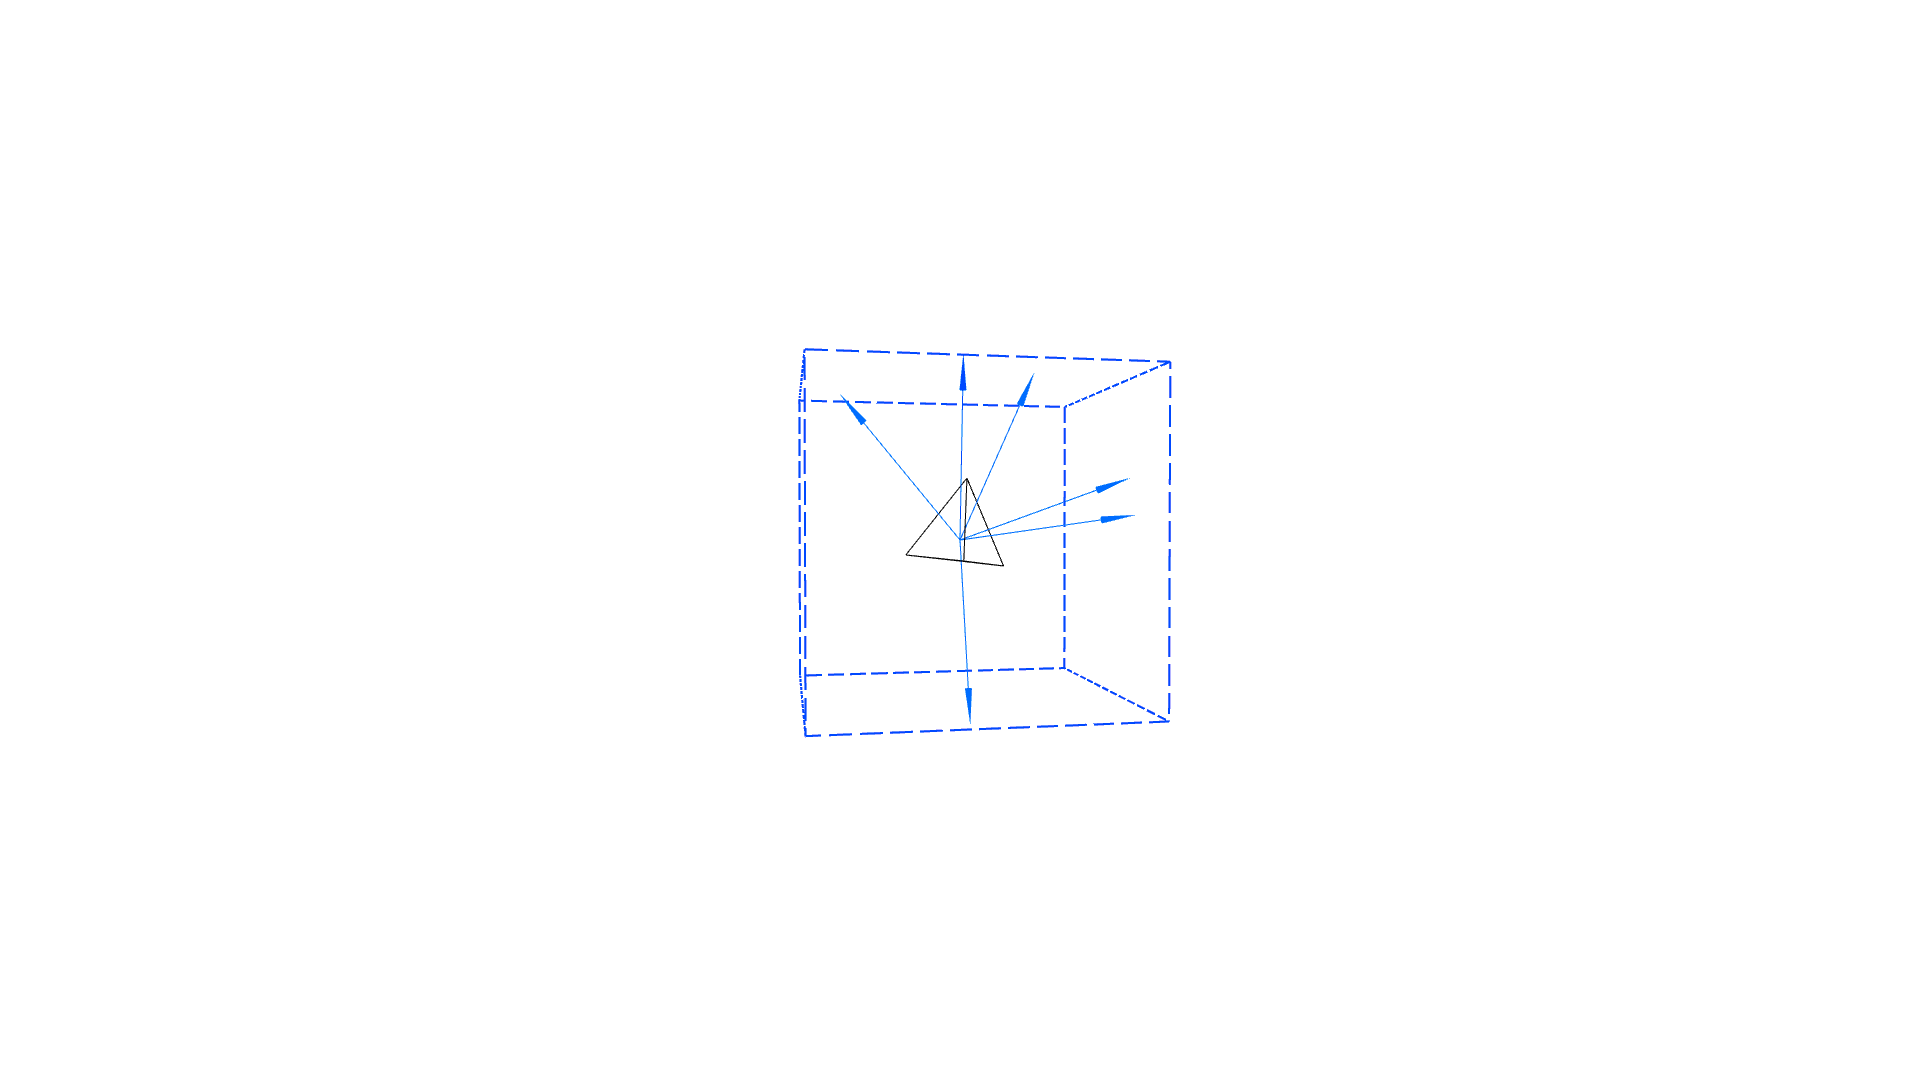
\includegraphics[width=0.49\textwidth]{img/output}
	\caption{Screenshot unseres Beispiel-Ausgabemoduls}
	\label{fig:output}
\end{wrapfigure}
Wir haben ein Beispiel-Ausgabemodul in Javascript implementiert. Mit diesem ist es möglich, die Positionsdaten zu visualisieren, was das unmittelbare Evaluieren stark vereinfacht. Die Programmiersprache Javascript haben wir gewählt, damit dieses Ausgabemodul auf jedem Endgerät mit modernem Webbrowser, wie z.B. Smartphones oder Laptops, ausgeführt werden kann.\\
Die Simulation enthält eine weitere Implementation eines Ausgabemoduls. Auch diese visualisiert die bestimmten Richtungen, erlaubt es aber, diese auf der gleichen Benutzeroberfläche wie die Sollrichtung anzuzeigen. Dies gibt ein sehr direktes Feedback beim Entwickeln des Algorithmus zur Richtungsbestimmung. Dieses letzte Modul könnte allerdings, dank unseres modularen Konzeptes, bei Bedarf auch anders, z.B. als Plugin für eine \textit{Digital Audio Workstation} (\textit{DAW}) implementiert werden.
\subsection{Testen der einzelnen Module}
Ein weiterer Vorteil der Modularität ist, dass jedes Modul unabhängig von den anderen Modulen funktionsfähig ist. Dadurch kann die korrekte Funktionsweise für jedes Modul einzeln überprüft werden und man kann Fehler besser lokalisieren.
Die Audiosimulation haben wir mithilfe eines selbstgeschriebenem Plotting Programms überprüft. Dieses stellt die von der Audiosimulation versendeten Samples in Abhängigkeit der Zeit dar. Damit kann manuell die Phasendifferenz von dem Graphen abgelesen und mit dem erwarteten Wert verglichen werden.
\begin{figure} [H]
	\centering
  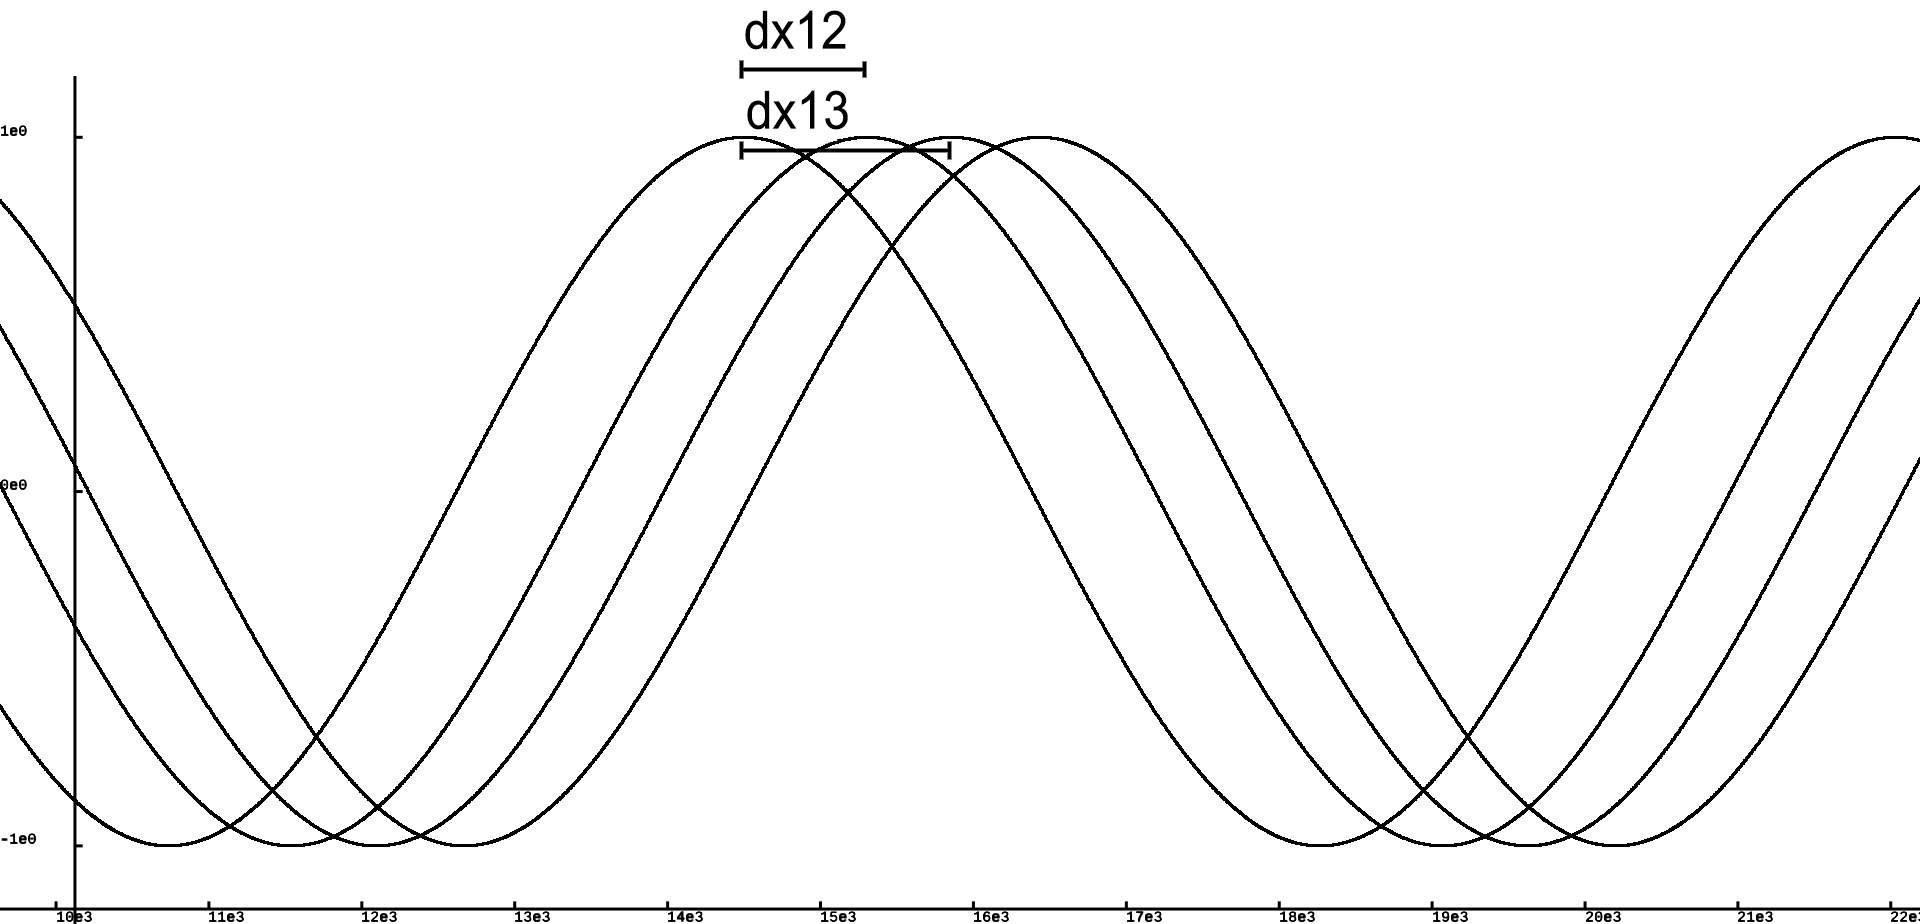
\includegraphics[width=.8\linewidth]{img/glplot}
  \caption{Screenshot unseres Plotting Programms}
  \label{fig:glplot}
\end{figure}

Die Fourier-Transformation konnten wir mit der vorher überprüften Audiosimulation testen. Dazu haben wir die von der Fourier-Transformation bestimmten Frequenz, Phase und Amplitude Tripel mit den tatsächlich in der Simulation eingestellten Werten verglichen.
Durch das Testen der einzelnen Module konnten wir effizient die vorhandenen Fehler, wie die falsche Berechnung der Phase und einen Fehler in der Distanzberechnung der Audiosimulation, finden und beheben.
